% GNUPLOT: LaTeX picture with Postscript
\begingroup
  \fontfamily{ptm}%
  \selectfont
  \makeatletter
  \providecommand\color[2][]{%
    \GenericError{(gnuplot) \space\space\space\@spaces}{%
      Package color not loaded in conjunction with
      terminal option `colourtext'%
    }{See the gnuplot documentation for explanation.%
    }{Either use 'blacktext' in gnuplot or load the package
      color.sty in LaTeX.}%
    \renewcommand\color[2][]{}%
  }%
  \providecommand\includegraphics[2][]{%
    \GenericError{(gnuplot) \space\space\space\@spaces}{%
      Package graphicx or graphics not loaded%
    }{See the gnuplot documentation for explanation.%
    }{The gnuplot epslatex terminal needs graphicx.sty or graphics.sty.}%
    \renewcommand\includegraphics[2][]{}%
  }%
  \providecommand\rotatebox[2]{#2}%
  \@ifundefined{ifGPcolor}{%
    \newif\ifGPcolor
    \GPcolortrue
  }{}%
  \@ifundefined{ifGPblacktext}{%
    \newif\ifGPblacktext
    \GPblacktexttrue
  }{}%
  % define a \g@addto@macro without @ in the name:
  \let\gplgaddtomacro\g@addto@macro
  % define empty templates for all commands taking text:
  \gdef\gplbacktext{}%
  \gdef\gplfronttext{}%
  \makeatother
  \ifGPblacktext
    % no textcolor at all
    \def\colorrgb#1{}%
    \def\colorgray#1{}%
  \else
    % gray or color?
    \ifGPcolor
      \def\colorrgb#1{\color[rgb]{#1}}%
      \def\colorgray#1{\color[gray]{#1}}%
      \expandafter\def\csname LTw\endcsname{\color{white}}%
      \expandafter\def\csname LTb\endcsname{\color{black}}%
      \expandafter\def\csname LTa\endcsname{\color{black}}%
      \expandafter\def\csname LT0\endcsname{\color[rgb]{1,0,0}}%
      \expandafter\def\csname LT1\endcsname{\color[rgb]{0,1,0}}%
      \expandafter\def\csname LT2\endcsname{\color[rgb]{0,0,1}}%
      \expandafter\def\csname LT3\endcsname{\color[rgb]{1,0,1}}%
      \expandafter\def\csname LT4\endcsname{\color[rgb]{0,1,1}}%
      \expandafter\def\csname LT5\endcsname{\color[rgb]{1,1,0}}%
      \expandafter\def\csname LT6\endcsname{\color[rgb]{0,0,0}}%
      \expandafter\def\csname LT7\endcsname{\color[rgb]{1,0.3,0}}%
      \expandafter\def\csname LT8\endcsname{\color[rgb]{0.5,0.5,0.5}}%
    \else
      % gray
      \def\colorrgb#1{\color{black}}%
      \def\colorgray#1{\color[gray]{#1}}%
      \expandafter\def\csname LTw\endcsname{\color{white}}%
      \expandafter\def\csname LTb\endcsname{\color{black}}%
      \expandafter\def\csname LTa\endcsname{\color{black}}%
      \expandafter\def\csname LT0\endcsname{\color{black}}%
      \expandafter\def\csname LT1\endcsname{\color{black}}%
      \expandafter\def\csname LT2\endcsname{\color{black}}%
      \expandafter\def\csname LT3\endcsname{\color{black}}%
      \expandafter\def\csname LT4\endcsname{\color{black}}%
      \expandafter\def\csname LT5\endcsname{\color{black}}%
      \expandafter\def\csname LT6\endcsname{\color{black}}%
      \expandafter\def\csname LT7\endcsname{\color{black}}%
      \expandafter\def\csname LT8\endcsname{\color{black}}%
    \fi
  \fi
  \setlength{\unitlength}{0.0500bp}%
  \begin{picture}(11320.00,3400.00)%
    \gplgaddtomacro\gplbacktext{%
      \colorrgb{0.50,0.50,0.50}%
      \put(918,680){\makebox(0,0)[r]{\strut{} 0}}%
      \colorrgb{0.50,0.50,0.50}%
      \put(918,1045){\makebox(0,0)[r]{\strut{} 0.1}}%
      \colorrgb{0.50,0.50,0.50}%
      \put(918,1411){\makebox(0,0)[r]{\strut{} 0.2}}%
      \colorrgb{0.50,0.50,0.50}%
      \put(918,1776){\makebox(0,0)[r]{\strut{} 0.3}}%
      \colorrgb{0.50,0.50,0.50}%
      \put(918,2141){\makebox(0,0)[r]{\strut{} 0.4}}%
      \colorrgb{0.50,0.50,0.50}%
      \put(918,2507){\makebox(0,0)[r]{\strut{} 0.5}}%
      \colorrgb{0.50,0.50,0.50}%
      \put(918,2872){\makebox(0,0)[r]{\strut{} 0.6}}%
      \colorrgb{0.50,0.50,0.50}%
      \put(1020,494){\makebox(0,0){\strut{} 0}}%
      \colorrgb{0.50,0.50,0.50}%
      \put(1897,494){\makebox(0,0){\strut{} 0.2}}%
      \colorrgb{0.50,0.50,0.50}%
      \put(2774,494){\makebox(0,0){\strut{} 0.4}}%
      \colorrgb{0.50,0.50,0.50}%
      \put(3650,494){\makebox(0,0){\strut{} 0.6}}%
      \colorrgb{0.50,0.50,0.50}%
      \put(4527,494){\makebox(0,0){\strut{} 0.8}}%
      \colorrgb{0.50,0.50,0.50}%
      \put(5404,494){\makebox(0,0){\strut{} 1}}%
      \csname LTb\endcsname%
      \put(315,1776){\rotatebox{-270}{\makebox(0,0){\strut{}Frequency}}}%
      \csname LTb\endcsname%
      \put(5589,1776){\rotatebox{-270}{\makebox(0,0){\strut{}}}}%
      \csname LTb\endcsname%
      \put(3212,215){\makebox(0,0){\strut{}E (GeV)}}%
      \put(3212,2779){\makebox(0,0){\strut{}}}%
      \csname LTb\endcsname%
      \put(3212,2778){\makebox(0,0){\strut{}}}%
      \put(408,178){\makebox(0,0)[l]{\strut{}}}%
      \put(3650,1776){\makebox(0,0)[l]{\strut{}decay to $\nu e^+ e^-$}}%
    }%
    \gplgaddtomacro\gplfronttext{%
      \csname LTb\endcsname%
      \put(4616,2612){\makebox(0,0)[r]{\strut{}100 MeV}}%
      \csname LTb\endcsname%
      \put(4616,2426){\makebox(0,0)[r]{\strut{}200 MeV}}%
      \csname LTb\endcsname%
      \put(4616,2240){\makebox(0,0)[r]{\strut{}350 MeV}}%
    }%
    \gplgaddtomacro\gplbacktext{%
      \colorrgb{0.50,0.50,0.50}%
      \put(6578,680){\makebox(0,0)[r]{\strut{} 0}}%
      \colorrgb{0.50,0.50,0.50}%
      \put(6578,1045){\makebox(0,0)[r]{\strut{} 0.05}}%
      \colorrgb{0.50,0.50,0.50}%
      \put(6578,1411){\makebox(0,0)[r]{\strut{} 0.1}}%
      \colorrgb{0.50,0.50,0.50}%
      \put(6578,1776){\makebox(0,0)[r]{\strut{} 0.15}}%
      \colorrgb{0.50,0.50,0.50}%
      \put(6578,2141){\makebox(0,0)[r]{\strut{} 0.2}}%
      \colorrgb{0.50,0.50,0.50}%
      \put(6578,2507){\makebox(0,0)[r]{\strut{} 0.25}}%
      \colorrgb{0.50,0.50,0.50}%
      \put(6578,2872){\makebox(0,0)[r]{\strut{} 0.3}}%
      \colorrgb{0.50,0.50,0.50}%
      \put(6680,494){\makebox(0,0){\strut{} 0}}%
      \colorrgb{0.50,0.50,0.50}%
      \put(7557,494){\makebox(0,0){\strut{} 0.2}}%
      \colorrgb{0.50,0.50,0.50}%
      \put(8434,494){\makebox(0,0){\strut{} 0.4}}%
      \colorrgb{0.50,0.50,0.50}%
      \put(9310,494){\makebox(0,0){\strut{} 0.6}}%
      \colorrgb{0.50,0.50,0.50}%
      \put(10187,494){\makebox(0,0){\strut{} 0.8}}%
      \colorrgb{0.50,0.50,0.50}%
      \put(11064,494){\makebox(0,0){\strut{} 1}}%
      \csname LTb\endcsname%
      \put(5873,1776){\rotatebox{-270}{\makebox(0,0){\strut{}Frequency}}}%
      \csname LTb\endcsname%
      \put(11249,1776){\rotatebox{-270}{\makebox(0,0){\strut{}}}}%
      \csname LTb\endcsname%
      \put(8872,215){\makebox(0,0){\strut{}E (GeV)}}%
      \put(8872,2779){\makebox(0,0){\strut{}}}%
      \csname LTb\endcsname%
      \put(8872,2778){\makebox(0,0){\strut{}}}%
      \put(5966,178){\makebox(0,0)[l]{\strut{}}}%
      \put(9310,1776){\makebox(0,0)[l]{\strut{}decay to $\nu e^+ e^-$}}%
    }%
    \gplgaddtomacro\gplfronttext{%
      \csname LTb\endcsname%
      \put(10276,2612){\makebox(0,0)[r]{\strut{}100 MeV}}%
      \csname LTb\endcsname%
      \put(10276,2426){\makebox(0,0)[r]{\strut{}200 MeV}}%
      \csname LTb\endcsname%
      \put(10276,2240){\makebox(0,0)[r]{\strut{}350 MeV}}%
    }%
    \gplbacktext
    \put(0,0){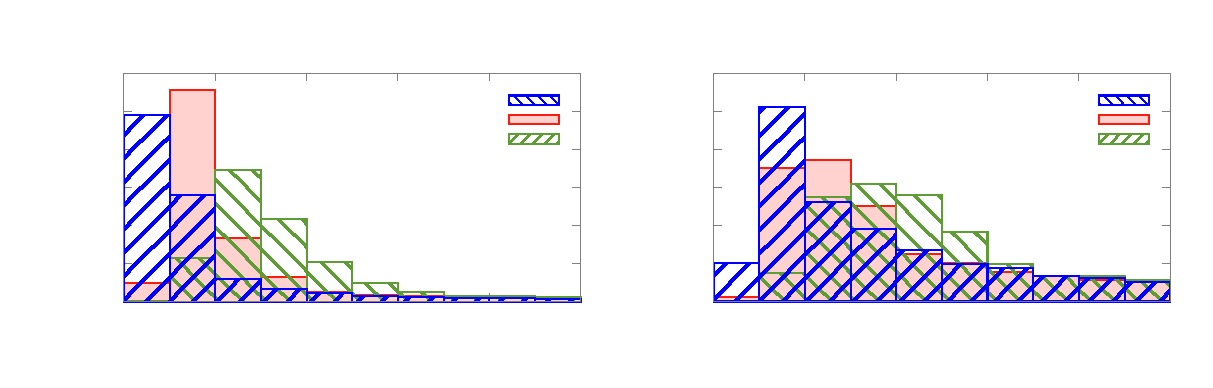
\includegraphics{figures/spectrum}}%
    \gplfronttext
  \end{picture}%
\endgroup
